\documentclass[a4paper,spanish] {article} 
\usepackage [spanish] {babel} 
\usepackage [latin1]{inputenc}
\usepackage{graphicx}
\usepackage{caratula}
\usepackage{subfig}
\usepackage{dsfont}
\usepackage{algorithm}
\usepackage{amsmath}
\usepackage{algorithmic}

\addtolength{\oddsidemargin}{-1in}
\addtolength{\textwidth}{2in}

\begin{document}
\pagestyle{headings}



\newpage

\materia{Aprendizaje por Refuerzos: Teoría y Aplicaciones en Robótica, Psicología y Neurociencias}
\submateria{Tp Final}
\titulo{Desarrollo de algoritmos de aprendizaje y análisis de resultados en una adaptación del problema Bomberman}

\integrante{Pablo Brusco}{527/08}{pablo.brusco@gmail.com}
\integrante{Carolina Hadad}{367/08}{carolinahadad@gmail.com}
\integrante{Sergio Medina}{333}{@gmail.com}
\integrante{Santiago Palladino}{138/05}{spalladino@gmail.com}
\integrante{Andres Taraciuk}{333}{@gmail.com}


\maketitle

\section{Objetivo}
	En  este Trabajo Practico nos interesa analizar el desempeño de los algoritmos de aprendizaje aprendidos durante el curso,  aplicándolos  en un problema distinto de los vistos. En nuestro caso, elegimos adaptar el juego del Bomberman. 
	
	Compararemos los resultados del aprendizaje en agentes model-free y model-based, con los algoritmos de QLearning, RMax, RMax Factorizado, Sarsa y Sarsa Lambda, mostrando cuáles de ellos funcionan mejor en nuestro caso y a qué se debe esto. Además analizaremos el efecto de aplicar rewards intermedios en el tiempo de aprendizaje del agente.
	
	Además veremos como varia el aprendizaje del agente al moverse en un ambiente estocástico con mayor o menor grado de aleatoriedad.

\section{Introducción}
	\subsection{Adaptación del juego del Bomberman}
	El juego que vamos usar es una versión simplificada del juego del Bomberman. El objetivo del agente es llegar a la salida. El agente tiene 4 acciones de movimiento: arriba, abajo, hacia la izquierda y hacia la derecha. El tablero tiene paredes que obstaculizan su camino, algunas de ellas son rompibles y otras irrompibles. El agente tiene acciones para poner una bomba y para explotarla. Solo puede haber una bomba en el tablero, si el agente realiza una acción de tirar bomba habiendo una bomba en el juego, la acción no tendrá efecto. Al explotar la bomba se destruirán las paredes que estén arriba, abajo a la izquierda y a la derecha de ella. Si el agente estuviera en alguno de estos lugares o sobre la bomba, el agente muere, teniendo que empezar el juego nuevamente desde la posición inicial. Nos interesa que el agente aprenda una política para llegar a la salida realizando la menor cantidad de acciones posibles.
	\subsection{Modelo Conceptal de la arquitectura}
	%pagina http://yuml.me/diagram/scruffy/class/draw
	%codigo [Manager| run()]->1[Task|start(); perform(action)]
	%		[Task] ->1[Environment|start(); performAction(action)]
	%		[Manager]->1[Agent | learn(); nextAction()]
	
	\begin{figure}[h!]
  \centering
    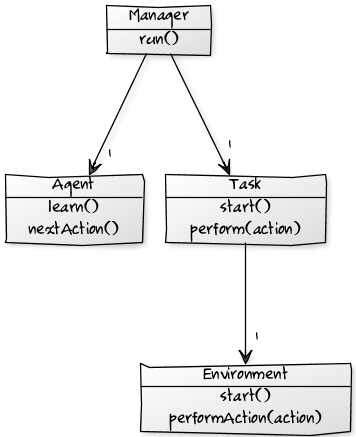
\includegraphics[width=0.5\textwidth]{MCarquitectra.png}
  \caption{Modelo Conceptual Arquitectura.}

\end{figure}
	
	
	\subsection{Uso}
	\subsection{Visualización}
	
\section{Algoritmos de Aprendizaje}
	Programamos agentes con políticas de aprendizaje distintas 
	\subsection{Agentes Model-Free}
		\subsubsection{QLearning}
		\subsubsection{Sarsa}
		\subsubsection{Sarsa ($\lambda$)}	
	\subsection{Agentes Model-Based}	
		\subsubsection{R-max}
		\subsubsection{R-max factorizado}

\section{Ambiente Estocastico}
	\subsection{Resultados}
	
 \section{Políticas de Refuerzo}
 	Para evaluar el efecto de aplicar políticas de refuerzos intermedios en el tiempo de aprendizaje de los agentes, incluimos los siguientes campos en el archivo de settings, que se agregan al refuerzo por llegar a la salida y al refuerzo negativo en el caso de que el agente muera. En el caso de que el agente llegue a la salida o muera recibe el WIN_REWARD o el LOSE_REWARD respectivamente, pero no se agrega este refuerzo adicional.

\begin{description}
\item[NAVIGATION_REWARD] 
	\begin{itemize}
	\item NAVIGATION_NO_REWARD: No se agrega refuerzos intermedios adicionales.
	\item NAVIGATION_REWARD_PROPORTIONAL_TO_EXIT : Siempre que el agente realice una acción que cambie su posición recibe un refuerzo adicional proporcional a su distancia a la salida. En el caso de las acciones de movimiento que no cambien el estado, como por ejemplo intentar moverse hacia una posición que tenga una pared, el agente no recibirá ningun refuerzo, de manera de desalentar este tipo de acciones. 
	
	Las formula para el cálculo de este refuerzo intermedio es la que sigue:
	$$ refuerzo = cercania_en_x + cercania_en_y $$
	donde
	$$ cercania_en_x =\mid MAP_SIZE-1 -(EXIT_0 - agentPosition_0) \mid$$
	$$ cercania_en_y =\mid MAP_SIZE-1 -(EXIT_1 - agentPosition_1) \mid$$
	siendo $EXIT = (EXIT_0, EXIT_1)$ la posición de la salida en el tablero y $ agentPosition= (agentPosition_0, agentPosition_1)$ la posición del agente.
	
	Por ejemplo para un tablero de $8 \times 8$ con la salida en $(7,7)$ los refuerzos que recibiría el agente al llegar a cada posición serían estos:
	\begin{figure}[h!]
  \centering
    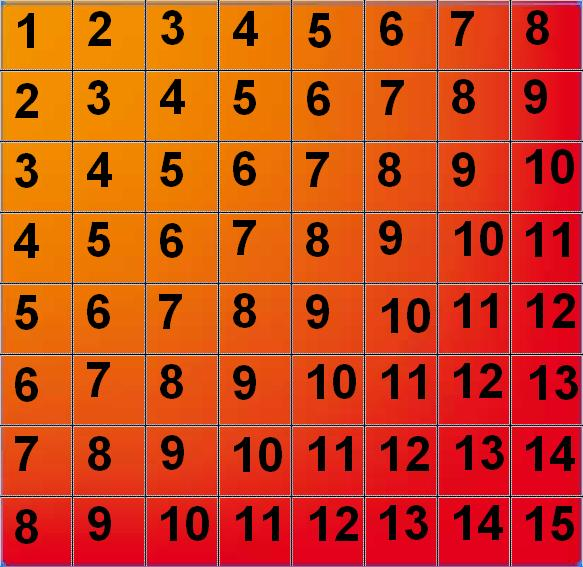
\includegraphics[width=0.5\textwidth]{refuerzos.jpg}
  \caption{Refuerzos para un tablero de 8 por 8 con salida en (7,7).}
	\end{figure}	
	La motivación de este refuerzo es que el agente trate de dirigirse hacia la salida.
	\end{itemize}

\item[BOMB_REWARD_POLICY] 
	\begin{itemize}
	\item BOMB_NO_REWARD: No se agrega refuerzos intermedios adicionales.
	\item BOMB_REWARD_PER_STONE_DESTROYED: Cada vez que el agente destruye una pared, sin morir, recibe un refuerzo igual al BOMB_REWARD del archivo de settings. La idea de este refuerzo es que el agente aprenda que debe destruir paredes.
	\item BOMB_REWARD_PER_STONE_DESTROYED_PROPORTIONAL_TO_EXIT: el refuerzo anterior, usado solo podría hacer que el agente, por lo menos en las primeras iteraciones, intente romper muchas paredes. Por eso agregamos esta opción, que le da mayor valor a romper paredes cercanas a la salida. La formula para este valor es $BOMB_REWARD \times cercania_a_la_salida$ calculando la cercanía de la misma forma que antes.
	
\item[NO_ACTION_NEGATIVE_REWARD] Para desalentar el que el agente realizara acciones que no modificaran el estado, agregamos este booleano. Si se activa, cada vez que el agente realiza una acción sin efecto, se le da un refuerzo negativo. 

\item[INITIAL_REWARD] En la misma línea que el ítem anterior, también permitimos variar el refuerzo que se le da al agente al realizar cualquier acción. La idea es que si este valor fuera negativo, el agente intentará llegar lo mas rápido a la salida. Esta idea se integra al $\gamma$, pero permite explicitar el valor negativo de realizar acciones.

	\end{itemize}

	


\end{description}

	Las funciones para la aplicación de estos refuerzos se pueden encontrar en el archivo $Rewards.py$ y son llamadas desde Task de acuerdo a las políticas elegidas por el usuario en el archivo de Settings.
 
	



\section{Pruebas y resultados}
	\subsection{Sin Rewards Intermedios}
	\subsection{Rewards Intermedios por posición del bomberman}
	\subsection{Rewards Intermedios por explotar bomba}
	\subsection{Rewards Intermedios por explotar bomba relativo a la posicion de la bomba}

\section{Conclusiones}


	





		


		
		

		
		
		
		
\newpage
\tableofcontents
\newpage
	 
	
\end{document}